\section{偏移与速度佶计}
\label{sec:3.6}

我们经常会同时面鞍倾角、炮检距及速度未知这三种复杂情况,告速度已知时,双平方
根方程提供了一个颇有吸引力的解决难题之途径。可是当速度朱知时,可就把人难住了,采
用上一节中所述那样的速度估计姓理办法吧,可它却又是假设没有倾角的情形。在这一节
中,我们将建立一神界面存在倾角时进行速度估计的方法。

\subsection{倾角时差校正---Sherwood的“魔鬼”方法}
\label{sec:3.6.1}

倾斜地层与水平方向的交角为$\alpha$时,Levin关于该倾斜层的反射旅行时间$t$的表达式为
(见\ref{sec:3.2}节)
\begin{equation}
t^2v^2=4(y-y_0)^2sin^2\alpha + 4h^2cos^2\alpha
\label{eq:ex3.6.1}
\end{equation}

在炮检距与时间的空间$(h,t)$内,这是一支双曲线。以$cos\alpha$为比例系数将速度$v$放大,
可使这时距曲线同无倾角情形下的时距曲线完全相同\footnote{
以$v/cos\alpha$代替$v$时,即得这种结果。---译者
}。常规处理办法就是沿这种曲线进行
叠加和速度分析,它常常能有满意结果。有时,结果却不令人满意,因为倾角不婊空间的单
值函数,例如,断层面附近将会存在绕射,这时它们是所有倾斜同相轴的叠加结果,每个同
相轴强度一般均比反射要弱。在同一位置上可以存在许多同相轴倾角,这会使速度沽计和叠
加受到干扰。

原则上,叠前偏移---它是完整的双平方根方程的某类实现方法---可以解决这种普遍
性问题,但是,从何处取得用于偏移方程中的速度呢?尽管仅在涉及小角度时,偏移对速度
有点不灵敏,而当所涉及的是广角时,偏移对速度就变得比较灵敏了。

应当考虑一下偏移处理能否与速度估计处理混合使用。J.W.C. Sherwood(1976)曾
经指出偏移与速度估计这两种处理究竟应该如何混合使用。应当把时差校正分为两部分考
虑。一部分与炮检距有关,即正常时差校正(NMO);另一部分则与倾角有关,这后一部
分处理在概念上是新颖的。Sherwood将该种与倾角有关的处理描述为一类滤波处理,但他
并未提供方法实现的细节。他把他的处理方法称作Devilish(
“魔鬼”方法),这个词是“dipping-event velocity inequalities licked”(倾斜同相轴速度不等量修正)的缩写。以后
Yilmaz更为实用性地把该种处理称为叠前局部偏移,但是最后终究还是把这种处理直接称为
倾角时差校正(dip moveout or
DMO)。我们将首先看一下Sherwood所得结杲,然后讨论
Rocca的倾角时差校正概念模型,最后是对两种概念上有区别的处理方法进行定量说明。

\begin{figure}[H]
\centering
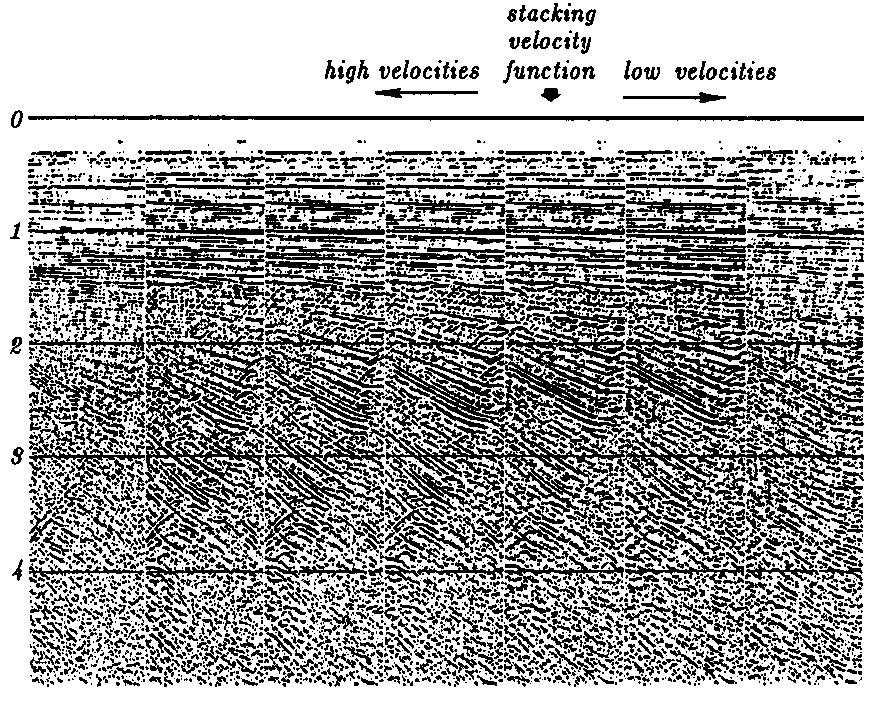
\includegraphics[width=0.65\textwidth]{vdmo/digicon}
\caption[digicon]{常规叠加速度扫描(Digicon公司提供)}
\label{fig:vdmo/digicon}
\end{figure}

图\ref{fig:vdmo/digicon}是叠加剖面的一小部分,这一部分在图中重复了若干次,每次采用的叠加速度
是不同的。要注意图中的特点,采用低速时,水平同相轴占优势;采用高速时,陡倾斜同相
轴占优势。在应用Devilish校正之后,像从前一样重新将数据叠加,结果如图\ref{fig:vdmo/rocca}所示,
这时叠加速度不再与倾角有关了。这意味着,在Devilish校正处理之后,测定速度能够无需
考虑倾角了,换句话说,所有各种倾角的同相轴对始终如一的相同速度都起作用,而不是每
一种倾斜同相轴各自预承心一种不同的速度。因此,Devilish这种校正处理对于具有相交同
相轴的资料理应能够提供更佳的速度,从而我们也就可以期望得到更好些的最终叠加结果。

\begin{figure}[H]
\centering
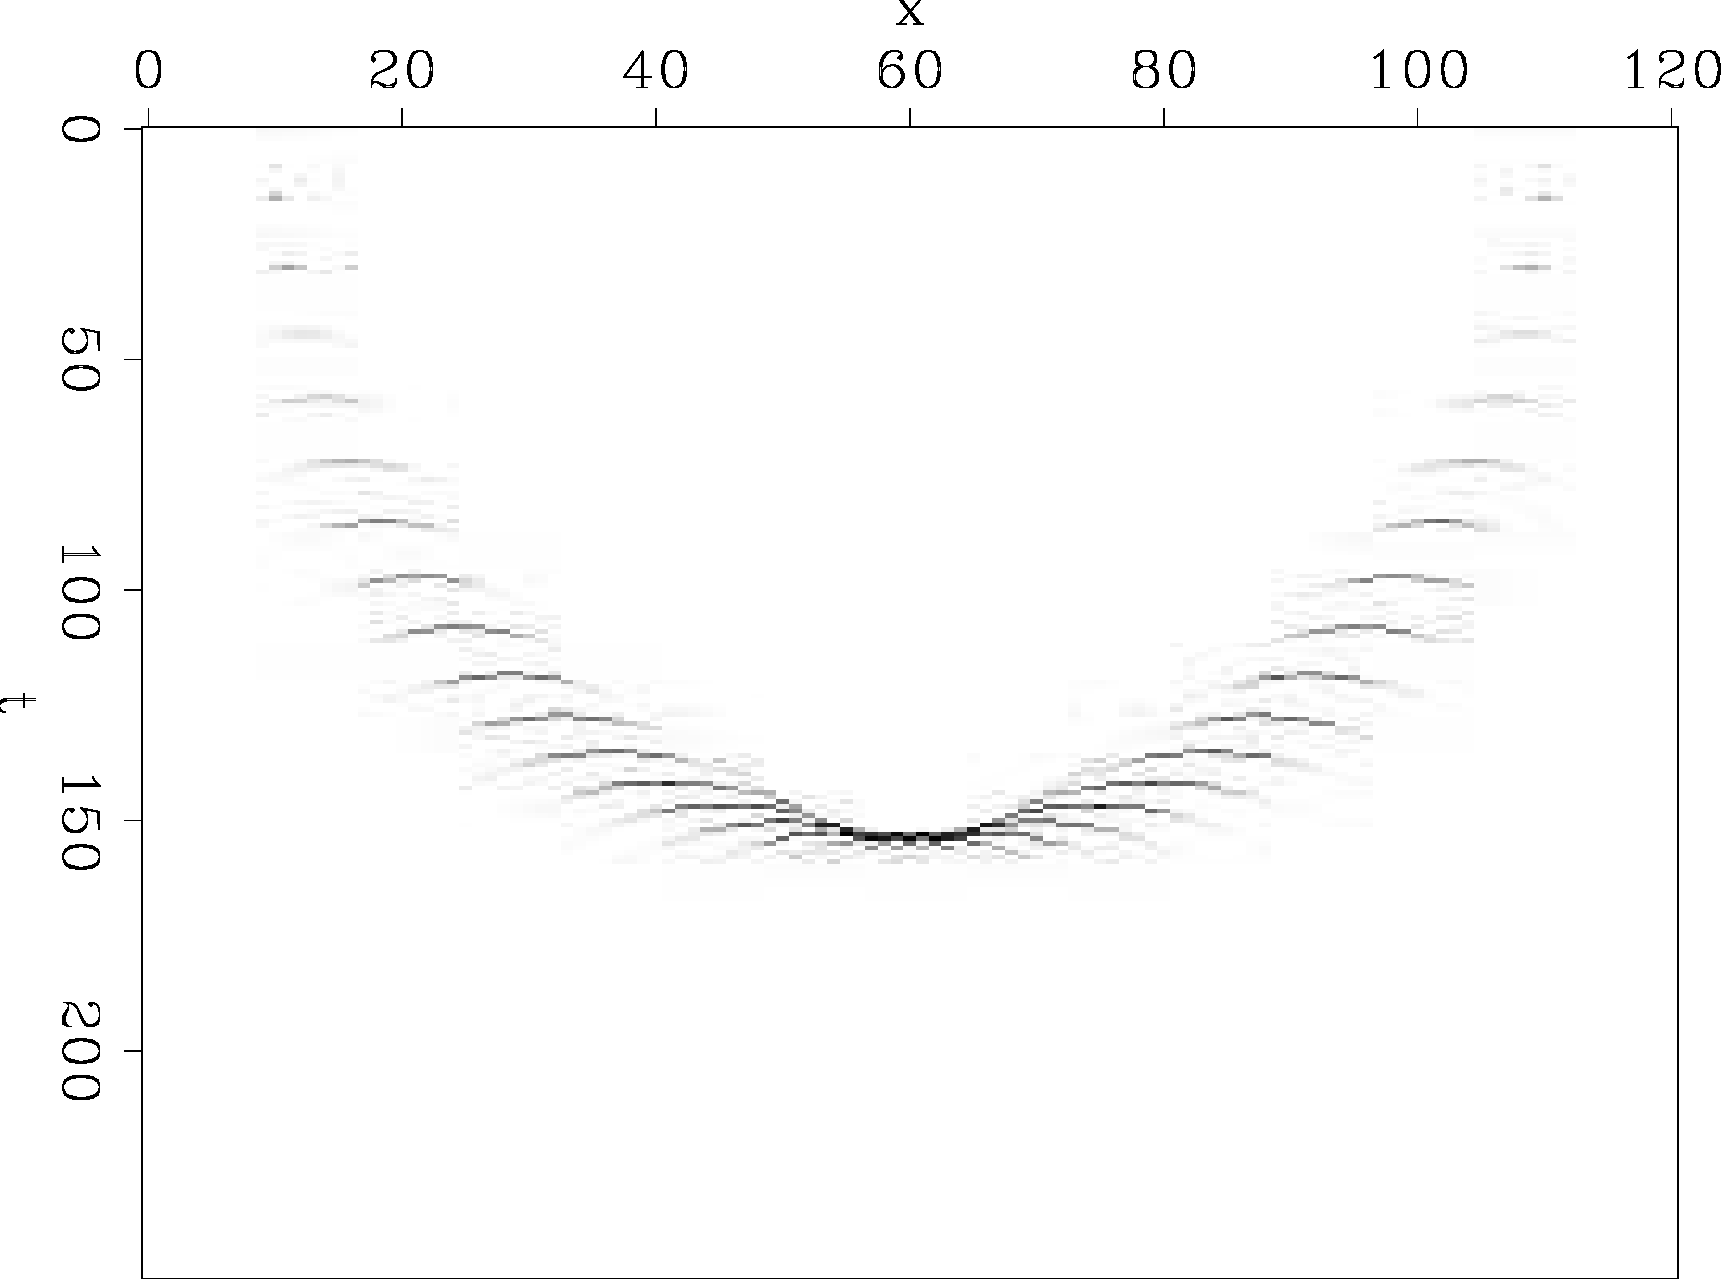
\includegraphics[width=0.65\textwidth]{vdmo/rocca}
\caption[rocca]{Rocca叠前局部偏移算子就是一种双曲线叠加,各该双曲线之顶点均位于半椭圆上。
将Rocca算子遍及中心点应用于共炮检距剖面,就可将该剖面转换为零炮检距剖面。
(据Gonzalez)}
\label{fig:vdmo/rocca}
\end{figure}

\subsection{Rocca的扫描算子}
\label{sec:3.6.2}

Fabio Rocca为Sherwood的倾角校正方法建立了一种概念清晰明确的摸型,现在用图
\ref{fig:vdmo/rocca2}来阐明Rocca的叠前局部偏移算子(prestack partial-migration operator)的概念。
试想像有一种在某个特定点$(t_0,y_0)$上含有一个脉冲函数的共炮检距剖面$P(t,y,h=h_0)$。其中,$t$为反射时间,
$y$为中心点坐标,$h_0$是该剖面所相应的固定炮检距。由于只有
$(t_0,y_0)$一个点上才有反射脉冲,这种资料所暗示的地层模型应是一个形状如半椭圆的反
射面,炮点在该椭圆的一个焦点上,接收点位于另一焦点上。根据这种地层模型,采用正演
模拟方法可作出一个相应的零炮检距剖面来,就是说,将半椭圆上的每一点扩展成双曲线,
即可得出零炮检距剖面。将共炮检距偏移和零炮检距绕射这两种运算结合起来,就得出了
Rocca算子。

\begin{figure}[H]
\centering
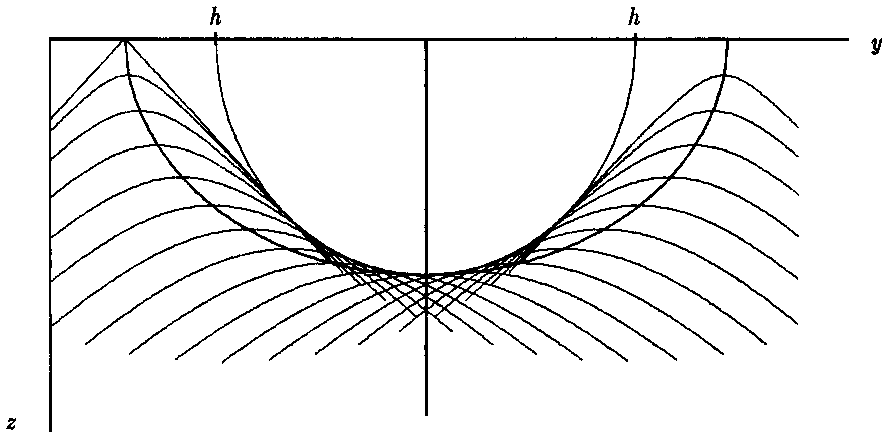
\includegraphics[width=0.65\textwidth]{vdmo/rocca2}
\caption[rocca2]{Rocca微笑曲线(据Ronen)}
\label{fig:vdmo/rocca2}
\end{figure}

Rocca算子就是图\ref{fig:vdmo/rocca}中的密切曲线(curve of osculation),
即各双曲线彼此得到
増强之处的微笑曲线(smile-shaped curve)\footnote{
该曲线状似人们微笑时的嘴,是以得名。---译者
}。如在椭圆弧上处处作出如图\ref{fig:vdmo/rocca}所示的
许多双曲线,而不是在几个孤立的点上作双曲线的话,这时该密切曲线就会在图上成为仅有
可见的东西了(而且还使你看不出它是从何而来)。

Rocca微笑曲线弧所相应之旅行时间的解析表达式表明,该弧是位于图\ref{fig:vdmo/rocca2}所示的一
个扃椭圆的末端部分。我们将略去这个微笑曲线方程的导出过程,最终可证明该方程为
\begin{equation}
\frac{(y-y_0)^2}{h^2}+\frac{t^2}{t_0^2} 
\label{eq:ex3.6.2}
\end{equation}
从这十方程看,Rocca算子好像是同速度无关似的。其实,它并不完全如此,因为微笑曲线
是在满足$dt/dy=2/v$关系的点上才截止的。

Rocca算子把共炮检距剖面变换成为零炮检距剖面,这种变换过程达到两个目的:第
一,它完成正常时差校正;第二,它完成Sherwood倾角校正。沿共炮检距剖面的中心点坐
标轴进行如图\ref{fig:vdmo/rocca}所示的运算,只在一个时间$t_0$上得出零炮检距剖面作为输出。对于每一
个时间$t_0$必须设计出不同的Rocca算子,所有$t_0$值时得出的输出必须叠加起来。图\ref{fig:vdmo/dmopoint}所
示就是若干$t_0$值时的若干个Rocca微笑曲线之叠加结果。

\begin{figure}[H]
\centering
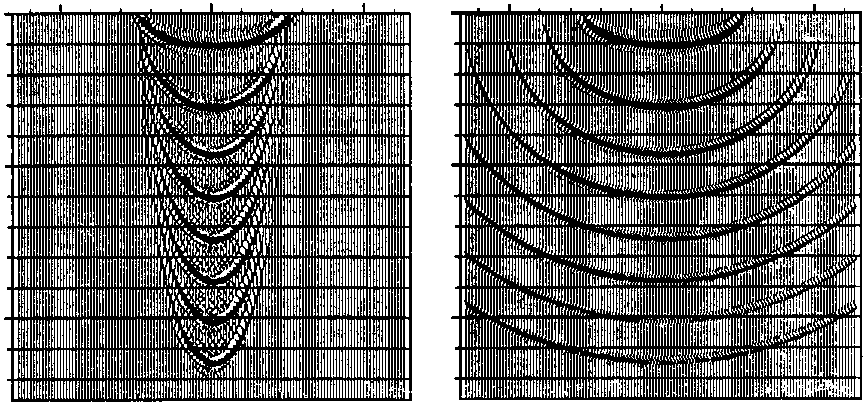
\includegraphics[width=0.65\textwidth]{vdmo/dmopoint}
\caption[dmopoint]{倾角时差校正之点源响应(左图)与共炮检距偏移扫描(右图)的比较(据Hale
)}
\label{fig:vdmo/dmopoint}
\end{figure}

从实用的观点看,这种算子特别有吸引力,因为对各个共炮检距剖面进行偏移处理时,
不是利用大而宽的椭圆进行大数据量处理,而只需要狭而小的Rocca算子。由图\ref{fig:vdmo/dmopoint}可
知,倾角时差校正算子\footnote{
文中所述倾角时差校正算子(dip moveout operator)、
Rocca微笑曲线、Rocca算子,Rocca叠前局部偏移
算子,密切曲线等等,大体均指同一类运算。---译者
}内的能量集中于该曲线底部附近很狭的范围内;在极限情形下,半
椭圆趋近于半圆,那就是说,在值较小的情形下,能量全部趋向底部。当所有能量集
中于底部一个点附近时,该Rocca算子实际上就变成一个$\delta$函数。在各炮检距均被校正为零
炮检距情形之后,根据正常时差剩余校正确定速度,然后再将数据叠加并偏移。

Rocca椭球体的扁度(narrowness
)在两种意义上有好处,从实用上说,它意味着在完
成速度估计和叠加以前,不需要将很多的中心点资料数据输入于计算机内存;更为重要的
是,由于算子所需的运算如此简洁紧凑,它确实不必对数据作大量运算。这点好处很重要,
因为运算是在完全已知速度之前的早期阶段完成的,所以有可能令人满意地选取区域性的恒
定值、例如取2.5公里/秒作为Rocca算子所需的速度值。

若有倾角时差校正算子的旅行时间曲线表达式,可能会有助于Kirchhoff积分求和型的
偏移扫描勉理,这将要求某些代数推导演绎,由此可导至Ottolini与Hale所建立算子牟身的
Fourier变换表现形式。

\subsection{Hale的共炮检距倾角时差校正}
\label{sec:3.6.3}

Hale(1983年)求出了对共炮检距剖面进行运算的倾角时差校正之Fourier变换表达形
式。参阅下表所列各定义方程:
\begin{table}[!ht]
\centering
\ttfamily
\small
\begin{tabularx}{\textwidth}{|Y|Y|Y|}
\hline
正常时差校正(NMO)& $t\rightarrow t_n$ & $t=\sqrt{t_n^2+4h^2/v^2}$\\
\hline
Levin正常时差校正& $t\rightarrow t_0$ & $t=\sqrt{t_0^2+4h^2cos^2\alpha/v^2}$\\
\hline
倾角时差校正(DMO)& $t_n\rightarrow t_0$ & $t=\sqrt{t_0^2-4h^2sin^2\alpha/v^2}$\\
\hline
\end{tabularx}
\end{table}
将倾角时差校正(DMO)方程代入正常时差校正(NMO
)方程中,就得出Levin正常时差校正方程\footnote{
$t$为反射时间,$2h$为炮点至检波点的炮检距,$v$为地层速度,$\alpha$为地层倾角,$t_0$为中心点(炮点与检波点之间的中心
点)下之界面的双程垂直时间(垂直深度$vt_0/2$)。若炮点位于上倾方向,检波点位于下倾方向,则炮点下界面的
双程垂直时间为$t_0-2hsin\alpha/v$;检波点下之界面双程垂直时间为$t_0+2hsin\alpha/v$;,由此可知,时间$t_n$为上述两种垂直时间的几何平均值。---译者
}。

要利用上表中的倾角关系方程,需知地层倾角$\alpha$,该倾角可由零炮检距剖面测定。在
Fourier空间内的零炮检距剖面上,该倾角的正弦为$vk_y/2\omega$,其中$k_y$为沿中心点坐标$y$的空
间波数;为强调这种测定仅应用于零炮检距剖面,我们总将$\omega$写为$\omega_0$,即
\begin{equation}
sin\alpha = \frac{vk_y}{2\omega_0}
\label{eq:ex3.6.3}
\end{equation}

不存在倾角时,正常时差校正应将任何记录道转换成零炮检距记录道。类似地,存在倾角
时,正常时差校正与倾角时差校正联合应用将把任何共炮检距剖面转换为零炮检距剖面。按
这种方式由共炮检距剖面制造出来的拟零炮检距剖面(pseudo-zero-offset section)
将以$P_0(t_0,h,y)$表示。首先按中心点坐标$y$取其Fourier变换对偶$k_y$,然后遍及时间$t_0$取Four­ier
变换,得
\begin{equation}
P_0(\omega_0,h,k_y)=\int e^{i\omega_0t_0}P_0(t_0,h,k_y)dt_0
\label{eq:ex3.6.4}
\end{equation}
将积分变量由$t_0$改变为$t_n$,则
\begin{equation}
P_0(\omega_0,h,k_y)=\int \frac{dt_0}{dt_n}e^{i\omega_0t_0(t_n)}P_0(t_0(t_n),h,k_y)dt_0
\label{eq:ex3.6.5}
\end{equation}
用正常时差校正之后的资料$P_n$来表示被积函数,采用$P_n(t_n,h,k_y)=P_0(t_0(t_n),h,k_y)$的办法即可作到这点
\begin{equation}
P_0(\omega_0,h,k_y)=\int \frac{dt_0}{dt_n}e^{i\omega_0t_0(t_n)}P_n(t_n,h,k_y)dt_n
\label{eq:ex3.6.6}
\end{equation}
同采用Stolt偏移处理时一样,上述变换中与心$dt_0/dt_n$有关的Jacobi函数行列式对各项均起标
定作用,但是对时移则不起作用。倾角时差校正(DMO)实际上是利用指数项完成的。

略去该Jacobi函数行列式项(它将近为1,作用确实不大),整个处理过程可用程序概
略表示如下;
\begin{minted}{Fortran}
P(k_y)=FT[P(y)]
P_n(t_n)=NMO[P(t)]
for all k_y { #three nested loop, interchangeable
for all h   { #three nested loop, interchangeable
for all w_0 { #three nested loop, interchangeable
        sum=0
        for all t_n {
          sum=sum+exp[iw_0[t_n^2+h^2k_y^2/(w_0^2)]^(1/2)]P_n(t_n,h,k_y)
        }
        P_0(w_0,h,k_y)=sum
        }}}
p_0(t_0,h,y)=FT2D[P_0(w_0,h,k_y)]
\end{minted}
要注意,在程序的内-环中的指数项是与速度无关的.倾角时差校正方程(DMO)中
的速度在用式\ref{eq:ex3.6.3}代换$sin\alpha$以后就消失了,所以倾角时差校正并不依赖于速度。

以上概述的处理过程要求在倾角时差校正之前进行正常时差校正(NMO)。要是顺序颠
倒,就会成为一种近似方法。遗憾的是我们不得不这么颠倒,因为我们不知道速度,宁可在
需要进行速度佶计的正常时差校正(NMO)步骤之前来完成计算量大的这种与速度无关之
倾角时差校正(DMO))步骤。图\ref{fig:vdmo/dmoproc}为倾角时差校正处理结果。

\begin{figure}[H]
\centering
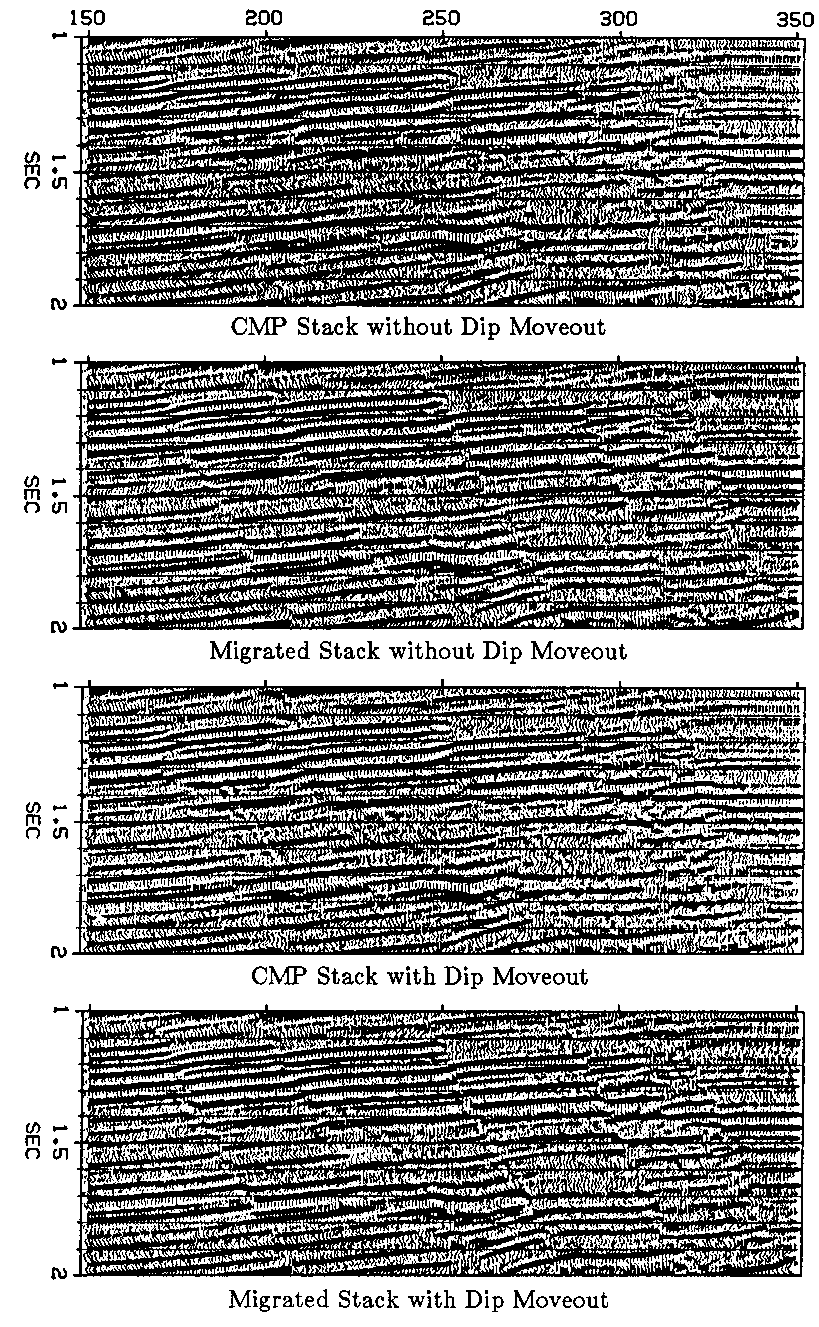
\includegraphics[width=0.65\textwidth]{vdmo/dmoproc}
\caption[dmoproc]{倾角时差校正处理的剖面(据Hale,1983
)}
\label{fig:vdmo/dmoproc}
\end{figure}

\subsection{Ottolini 的径向记录道(Radial trace)}
\label{sec:3.6.4}

普通我们都把共中心点道集看作是地震记录道的一个集合,即许多时间函数的集合,
每一个时间函数相应于某个特定的炮检距。但是,这种$(h,t)$数据空间能够以不同的坐
标系统加以表示。Turhan Taner所介绍的径向记录道系统是具有某些美妙属性的一种坐标
系统,在这类系统中,不是按恒定炮检距来取记录道,而是按恒定角度取记录道。这种思
想如图\ref{fig:vdmo/otto}所示。

除有某些以后将变得更明显的理论优点之外,这种系统还有一些实用优点,其中,值得
注意的是:
(1)各记录道均匀填满非零数据空间;
(2)在较小时间上,各记录道在短波长之处彼此紧靠近,而在长波长之处则分开较
宽;
(3)给定记录道上的能量代表波动沿一 固定角度方向的传播情况。

这最后一个特征对于具有多次反射的数据
特别重要(见\ref{sec:5.6}节),不过,就我们的讨论
目的而言,径向记录道的最佳属性还是另外一种。

\begin{figure}[H]
\centering
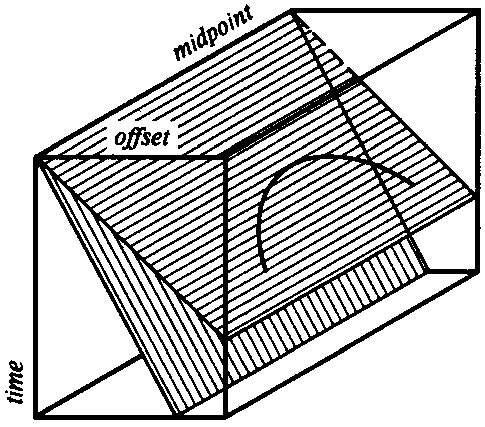
\includegraphics[width=0.65\textwidth]{vdmo/otto}
\caption[otto]{在反射地震侧线数据体积的内部,是称为径向记录道剖面的平面。
地层内部有一个点散射体,则径向记录道剖面上就有一支双曲线}
\label{fig:vdmo/otto}
\end{figure}

Richard Ottolini曾注意到,地层内的
点散射体在径向记录道剖面上表现为准确的双
曲线,而不是具有平缓顶部的双曲面。点散射
体的旅行时间曲线或Cheop金字塔形的曲线
族,可写成“弦长度”方程或扁圆方程(见
\ref{sec:3.2}节)。作下列定义
\begin{equation}
sin\phi = \frac{2h}{vt}
\label{eq:ex3.6.7}
\end{equation}
并代入\ref{sec:3.2}节中的式\ref{eq:ex3.2.13}内,得
\begin{equation}
vt=2[\frac{z^2}{cos^2\phi}+(y-y_0)^2]^{1/2}
\label{eq:ex3.6.8}
\end{equation}
用$cos\phi$来标定$z$轴,又完全重现圆和双曲线的情形!现将隐含的双曲緣表示成图\ref{fig:vdmo/ottohyp}中所
示的三维图像。

\begin{figure}[H]
\centering
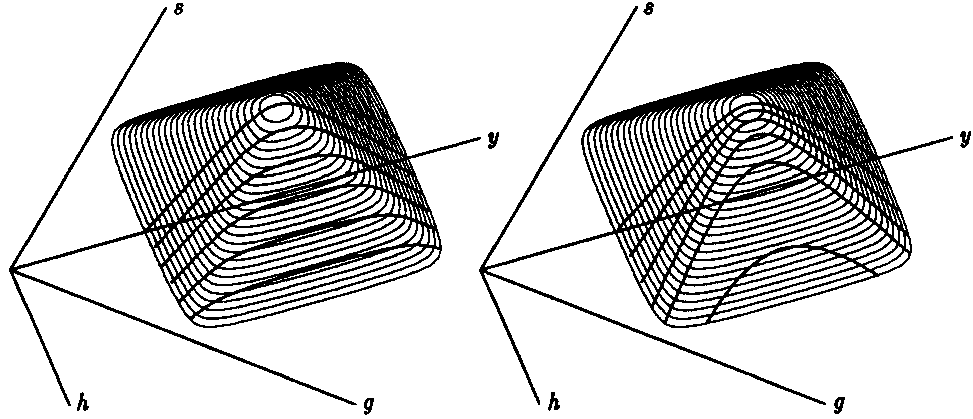
\includegraphics[width=0.65\textwidth]{vdmo/ottohyp}
\caption[ottohyp]{在Cheop金字塔中是平顶的双曲线,在径向记录道剖面上却是绕射双曲线}
\label{fig:vdmo/ottohyp}
\end{figure}

我们将会看到,图\ref{fig:vdmo/ottohyp}中的径向剖面内的双曲线比固定炮检距$h$时所看到的平顶双曲
面更容易掌握一些。参考下表定义倾角时差校正的方程和定义径向记录道坐标系内之普通的
时差校正的方程,就会明白这点。

下表中的第二个方裎就是零炮检距偏移采用的爆炸反射面方程,在双平方根方程中令
$H=0$也可以得出该式。如该式所示,它包含有地层速度而不是半速。方程\ref{eq:ex3.6.8}说明,用
$cos\phi$将$z$坐标轴加以标定,则不同分值时的各双曲线就全都联系在一起,具有同一个形式了。
根据Fourier变换理论,用一个除因子$cos\phi$对$z$进行标定就会相当于甩一个乘因子$cos\phi$将$k_z$
加以标定。这就意味着,上表第一个方程可以适用于径向记录道剖面上的偏移双曲线和绕射
双曲线\footnote{
这个方程即是径向记录道剖面信移与统射的频散方程,炮检距信息隐藏于角度参量命内。---译者}。
从第一个和第二个方程中消去$k_z$,得出上述$\omega\rightarrow\omega_0$时的第三个方程,这个方程把
所有炮检距(实际上就是任何径向角度)偏移至零炮检距的运算同后来在零炮检剖面上进行
绕射扫描的运算全结合在一起了,所以总效果就是炮检距延拓、即正常时差校正(NMO)
和倾角时差校正\footnote{
这个频散方程所描述的是将径向剖面转换为零炮检距平面的运箅过程,它将$\omega$转换为$\omega_0$,事实上就是将时间$t$转
换为中心点位置上的双程垂直时间$t_0$。---译者
}(DMO)。上表最后两个方程是把$\omega\rightarrow\omega_0$时的第三个方程分解成$\omega\rightarrow\omega_s$和
$\omega_s\rightarrow\omega_0$的两个相继过程,这两个处理过程像是DMO和NMO,但是运算均在径向空间内进
行。径向NMO是一种简单的时不变(time-invariant)拉伸,因此采用符号$\omega_s$。

同共炮检距剖面的情形不同,现在的径向空间之倾角时差校正是能够在进行拉伸、速度
估计这些步骤之前完成的。让我们来论证一下倾角时差校正确实真的与速度无关。将式\ref{eq:ex3.6.7}代入前述表格中的径向DMO变换,得到由时间$t$至拉伸时间的变换方程
\begin{equation}
\frac{h^2}{t^2}k_y^2+\omega_s^2=\omega^2
\label{eq:ex3.6.9}
\end{equation}
我们可观察到速度$v$已经在式\ref{eq:ex3.6.9}中消失掉了,所以径向坐标系中的倾角时差校正确实
不依赖于速度,进行倾角时差校正的处理$\omega\rightarrow\omega_s$并不要求有速度信息。径向坐标系提供的好
处就是这种计算量相当大的处理可以在进行速度估计$\omega_s\rightarrow\omega_0$之前来完成。

利用式\ref{eq:ex3.6.9},倾角时差校正过程$\omega\rightarrow\omega_s$可以很方便地采用一种Stolt型的算法来实现。

前面的分析均已假设速度为常数。在倾角时差校正之后,即将进行常规速度分析、叠加
和零炮检距偏移之前,可以采用有效的实用近似方法恢复为对速度$v(z)$随深度而变情形的分
析。

无论径向记录道方法还是Hale的共炮检距方法都能在恒定速度介质中准确地解决所有
角度问题,可是没有一种方法能准确处理速度分层情形下的问题,连能否作到这点也不清楚
---因为没有一种方法是源于双平方根方程的。Yilmaz(1979)关于DMO方面的工作是源
于双平方根方程的。所以他的方法对于速度分层情形可望是严格的,但是Yilmaz也不能避
免与角度有关的近似处理问题。因此,理论工作尚有待完成。

\subsection{倾角时差校正的抗假频特性}
\label{sec:3.6.5}

你可能会想,如果将空间$(y,h,t)$以采样间隔$\Delta y$沿$y$轴采样,则任何最终偏移剖面
$P(y,z)$将没有比$\Delta y$更高的空间分辨率了。其实情形并不这样。

此处起作用的基本原理自Shannon时代以来就已经知道了,如果一个时间函数及其导数
均按时间间隔$2\Delta t$进行采样,倘若信号的原始宽度低于$1/(2\Delta t)$,则它们就可以完全重
建。更一般性地说,如果一个信号用m个独立的滤波器来滤波,而且所得这m个信号均按间
隔来采样,则该信号就可以被恢复。

这里的问题是如何将这种概念应用于地震资料。基本信号是地层模型,它的各种不同滤
波后的形式就是共炮检距剖面。记住,当增大炮检距时,CDP叠加的反射点是移向上倾方向
的。进一步的细节可参阅Bolondi、Loinger和Rocca(1982)的论文,他们首次指出了倾角
时差校正的抗假频特性。在对三维地震资料的兴趣日益增大的这个时期,应该对倾角时差校
正的抗假频的特性给予特别的注意。




\subsection{习题}
\label{sec:3.6.6}

\begin{enumerate}
\item 试述Hale的倾角时差校正处理中Jacobi函数行列式的影响。

\end{enumerate}

